\subsection{Niveau 2 - Balayer}

\begin{center}
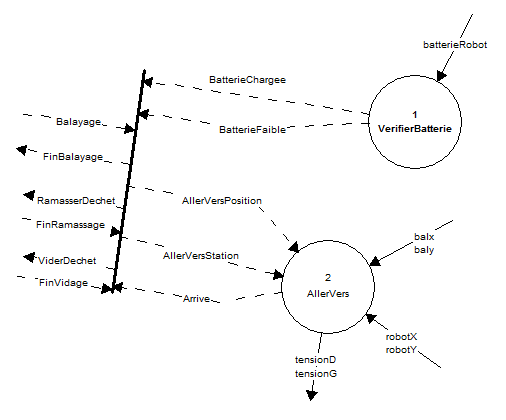
\includegraphics[scale=0.75]{\PIXPATH/balayer}
\end{center}


\subsubsection{Diagramme état-transition}

\begin{center}
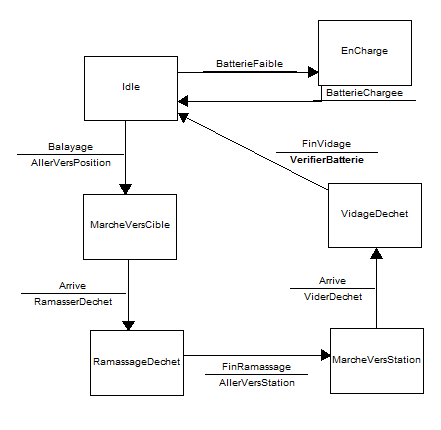
\includegraphics[scale=0.75]{\PIXPATH/balayer_etat}
\end{center}

\subsubsection{Processus primitifs - C-Spec}

\begin{description}
	
	\item \textbf{VerifierBatterie}
		\begin{tabbing} 
		\textbf{IN} : batterieRobot \\
		\textbf{OUT} : BatterieChargee, BatterieFaible \\
		si \=($batterieRobot \leq 0.15$) \\
			\>BatterieFaible emis \\
		sinon si ($batterieRobot \geq 0.95$ \\
			\>BatterieCahrgee emis \\
		fin si 
		\end{tabbing}


\end{description}

\vfill
\pagebreak

